\chapter{牛顿运动定律}
\section{牛顿第一、第三定律}


1.牛顿第一定律

(1)内容

一切物体总保持\_\_匀速直线运动\_\_状态或\_\_静止\_\_状态,直到有外力迫使它改变这种状态为止.

(2)意义

\ding{172}指出了一切物体具有\_\_惯性\_\_,因此牛顿第一定律又称\_\_惯性定律\_\_.

\ding{173}指出力不是\_\_维持\_\_物体运动状态的原因,而是\_\_改变\_\_物体运动状态的原因,即力是产生\_\_加速度\_\_的原因.

\ding{174}当物体不受力时,物体总保持\_\_匀速直线运动\_\_状态或\_\_静止\_\_状态.

(3)惯性

\ding{172}定义:物体具有保持原来\_\_匀速直线运动\_\_状态或\_\_静止\_\_状态的性质.

\ding{173}量度:\_\_质量\_\_是物体惯性大小的唯一量度,与物体的运动状态、受力情况、地理位置均无关,\_\_质量大\_\_的物体惯性大,\_\_质量小\_\_的物体惯性小.

\ding{174}普遍性:惯性是物体的\_\_固有\_\_属性,一切物体都有惯性.

2.牛顿第三定律

(1)作用力和反作用力

两个物体之间的作用总是\_\_相互\_\_的,一个物体对另一个物体施加了力,另一个物体同时对这个物体也施加了力.

(2)内容

两个物体之间的作用力和反作用力总是大小\_\_相等\_\_、方向\_\_相反\_\_、作用在\_\_同一条直线上\_\_.

(3)表达式

$F=-F^{\prime}$.

(4)意义

建立了相互作用物体之间的联系及作用力与\_\_反作用力\_\_的相互依赖关系.

\newpage
\subsection{牛顿第一定律的应用技巧}

1.应用牛顿第一定律分析实际问题时,要把生活感受和理论问题联系起来深刻认识力和运动的关系,正确理解力不是维持物体运动状态的原因,克服生活中一些错误的直观印象,建立正确的思维习惯.

2..如果物体的运动状态发生改变,则物体必然受到不为零的合外力作用.因此,判断物体的运动状态是否改变,以及如何改变,应分析物体的受力情况.

{[}例1{]}伽利略创造性地把实验、假设和逻辑推理相结合的科学方法,有力地促进了人类科学认识的发展,利用如图所示的装置做如下实验:小球从左侧斜面上的O点由静止释放后沿斜面向下运动,并沿右侧斜面上升.斜面上先后铺垫三种粗糙程度逐渐降低的材料时,小球沿右侧斜面上升到的最高位置依次为1、2、3.根据三次实验结果的对比,可以得到的最直接的结论是( A )

\begin{center}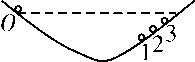
\includegraphics[width=0.88542in,height=0.28125in]{media/image95.png}\end{center}

A.如果斜面光滑,小球将上升到与O点等高的位置

B.如果小球不受力,它将一直保持匀速运动或静止状态

C.如果小球受到力的作用,它的运动状态将发生改变

D.小球受到的力一定时,质量越大,它的加速度越小
\begin{solution}
	根据题意,铺垫材料粗糙程度降低时,小球上升的最高位置升高,当斜面绝对光滑时,小球在斜面上没有能量损失,因此可以上升到与O点等高的位置,而B、C、D三个选项,从题目不能直接得出,所以选项A正确.
\end{solution}


\subsection{对牛顿第三定律的理解及应用}

1.相互作用力的特点:``三同、三异、三无关''.

(1)三同:同大小;同时产生、变化、消失;同性质

(2)三异:反向;异体,即作用力、反作用力作用在不同物体上;不同效果

(3)三无关:与物体的种类无关;与相互作用的两物体的运动状态无关;与是否和其他物体相互作用无关

2.一对平衡力与作用力、反作用力的不同点:

\begin{longtable}[]{@{}lll@{}}
\toprule


  & \begin{minipage}[b]{0.30\columnwidth}\raggedright
一对平衡力\strut
\end{minipage} & \begin{minipage}[b]{0.30\columnwidth}\raggedright
作用力与反作用力\strut
\end{minipage}\tabularnewline
\midrule
\endhead
作用对象 & 同一个物体 & 两个相互作用的不同物体\tabularnewline
作用时间 & 不一定同时产生、同时消失 &
一定同时产生、同时消失\tabularnewline
力的性质 & 不一定相同 & 一定相同\tabularnewline
作用效果 & 可相互抵消 & 不可抵消\tabularnewline
\bottomrule
\end{longtable}



\begin{center}
\includegraphics[width=0.70833in,height=0.125in]{media/image34.png}

\textbf{应用牛顿第三定律应注意的三个问题}
\end{center}


(1)定律中的``总是''说明对于任何物体,在任何情况下牛顿第三定律都是成立的.

(2)作用力与反作用力虽然等大反向,但因所作用的物体不同,所产生的效果(运动效果或形变效果)往往不同.

(3)作用力与反作用力只能是一对物体间的相互作用力,不能涉及第三个物体.
\newpage
\section{牛顿第二定律 两类动力学问题}


1.牛顿第二定律

(1)内容:物体加速度的大小跟它受到的作用力成\_\_正比\_\_,跟它的质量成\_\_反比\_\_.加速度的方向与\_\_作用力的方向\_\_相同.

(2)表达式:\_\_F=ma\_\_,F与a具有瞬时对应关系.

(3)适用范围:

\ding{172}牛顿第二定律只适用于\_\_惯性参考系\_\_(相对地面静止或做匀速直线运动的参考系).

\ding{173}牛顿第二定律只适用于\_\_宏观物体\_\_(相对于分子、原子)、\_\_低速运动\_\_(远小于光速)的情况.

2.动力学两类基本问题

(1)动力学两类基本问题

\ding{172}已知受力情况,求物体的\_\_运动\_\_情况.

\ding{173}已知运动情况,求物体的\_\_受力\_\_情况.

(2)解决两类基本问题的方法

以\_\_加速度\_\_为``桥梁'',由运动学公式和牛顿运动定律列方程求解,具体逻辑关系如图所示.

\begin{center}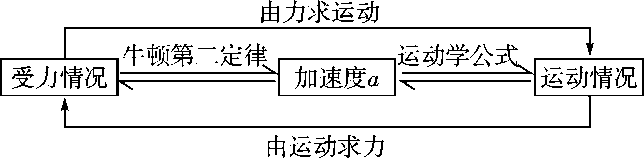
\includegraphics[width=2.92708in,height=0.71875in]{media/image99.png}\end{center}

\newpage
\subsection{牛顿第二定律的瞬时性}

\begin{center}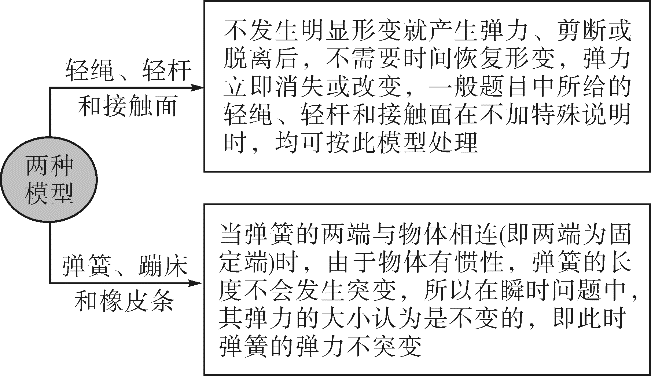
\includegraphics[width=2.95833in,height=1.70833in]{media/image100.png}\end{center}

{[}例1{]}(2018·广西南宁模拟)两个质量均为m的小球,用两条轻绳连接,处于平衡状态,如图所示.现突然迅速剪断轻绳OA,让小球下落,在剪断轻绳的瞬间,设小球A、B的加速度分别用$a_1$和$a_2$表示,则( A )

\begin{center}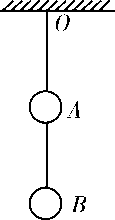
\includegraphics[width=0.3in]{media/image101.png}
	
\end{center}

A.$a_1$=g $a_2$=g

B.$a_1$=0 $a_2$=2g

C.$a_1$=g $a_2$=0

D.$a_1$=2g $a_2$=0

【拓展延伸1】把``轻绳''换成``轻弹簧''

在{[}例1{]}中只将A、B间的轻绳换成轻质弹簧,其他不变,如图所示,则典例选项中正确的是( D )

\begin{center}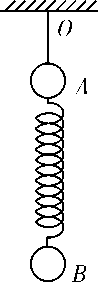
\includegraphics[width=0.3in]{media/image102.png}
	
\end{center}

A.$a_1$=g $a_2$=g

B.$a_1$=0 $a_2$=2g

C.$a_1$=g $a_2$=0

D.$a_1$=2g $a_2$=0



\begin{center}
\includegraphics[width=0.70833in,height=0.125in]{media/image13.png}

\textbf{抓住``两关键''、遵循``四步骤''}
\end{center}


(1)分析瞬时加速度的``两个关键''

\ding{172}明确绳或线类、弹簧或橡皮条类模型的特点.

\ding{173}分析瞬时前、后的受力情况和运动状态.

(2)``四个步骤''

第一步:分析原来物体的受力情况.

第二步:分析物体在突变时的受力情况.

第三步:由牛顿第二定律列方程.

第四步:求出瞬时加速度,并讨论其合理性.
\newpage
\subsection{动力学两类基本问题}

\begin{center}
\includegraphics[width=0.70833in,height=0.125in]{media/image25.png}

\textbf{动力学两类基本问题的解题思路}
\end{center}


\begin{center}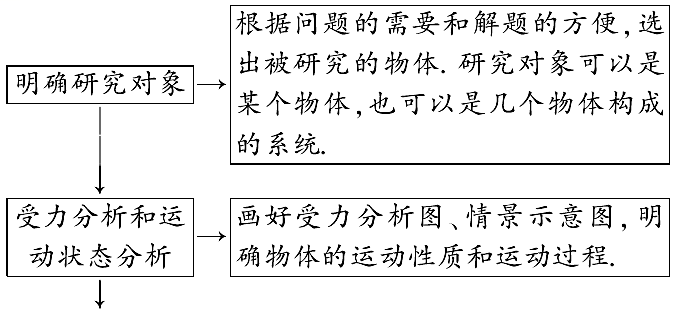
\includegraphics[width=2.94792in,height=1.35417in]{media/image104.png}\end{center}
\begin{center}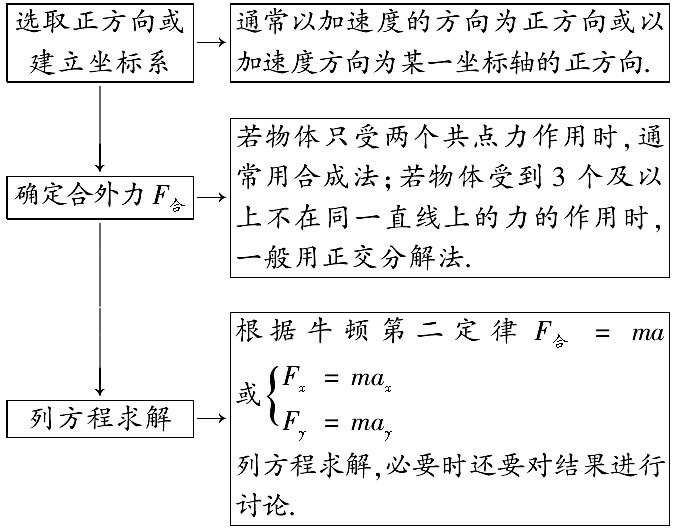
\includegraphics[width=2.94792in,height=2.32292in]{media/image105.png}\end{center}

{[}例2{]}(2018·广东深圳模拟)如图所示为四旋翼无人机,它是一种能够垂直起降的小型遥控飞行器,目前得到越来越广泛的应用.

\begin{center}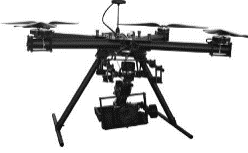
\includegraphics[width=1.125in,height=0.69792in]{media/image106.png}\end{center}

一架质量m=2 kg的无人机,其动力系统所能提供的最大升力F=36
N,运动过程中所受空气阻力大小恒为$F_f=4 N$,g取 $10m/s^2$.

(1)无人机在地面上从静止开始,以最大升力竖直向上起飞.求在t=5
s时离地面的高度h;

(2)无人机悬停在距离地面高度H=100
m处,由于动力设备故障,无人机突然失去升力而坠落.求无人机坠落地面时的速度v;

(3)在无人机坠落过程中,在遥控设备的干预下,动力设备重新启动提供向上最大升力.为保证安全着地,求飞行器从开始下落到恢复升力的最长时间t1.
\begin{solution}
	(1)75 m (2)40 m/s (3) $\dfrac{5\sqrt{5}}{3}$.
\end{solution}


\begin{center}
\includegraphics[width=0.70833in,height=0.125in]{media/image13.png}

\textbf{解决两类动力学问题的两个关键点}
\end{center}


(1)把握``两个分析''\,``一个桥梁''

两个分析:物体的受力情况分析和运动过程分析.

一个桥梁:加速度是联系物体运动和受力的桥梁.

(2)寻找多过程运动问题中各过程间的相互联系.如第一个过程的末速度就是下一个过程的初速度,画图找出各过程的位移之间的联系.

\subsection{等时圆模型及其应用}

1.模型特征

\begin{center}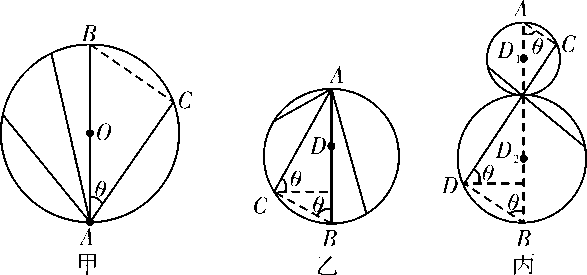
\includegraphics[width=2.66667in,height=1.25in]{media/image107.png}\end{center}

(1)质点从竖直圆环上沿不同的光滑弦上端由静止开始滑到环的最低点所用时间相等,如图乙所示;

(2)质点从竖直圆环上最高点沿不同的光滑弦由静止开始滑到下端所用时间相等,如图乙所示;

(3)两个竖直圆环相切且两环的竖直直径均过切点,质点沿不同的光滑弦上端由静止开始滑到下端所用时间相等,如图丙所示.

2.思维模板

\begin{center}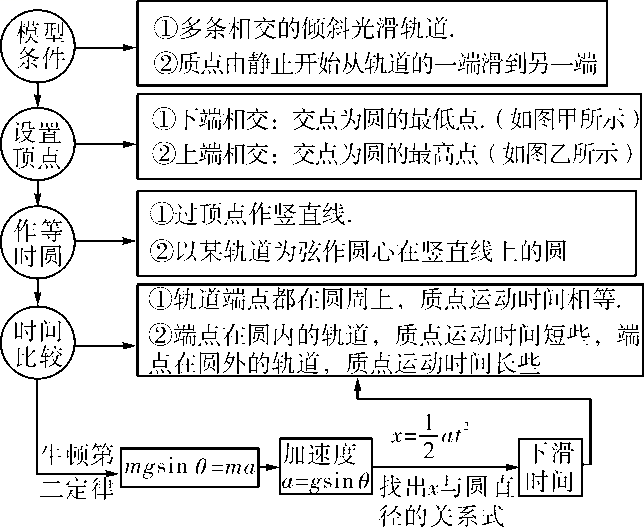
\includegraphics[width=2.92708in,height=2.39583in]{media/image108.png}\end{center}

{[}例3{]}(2017·山东济南模拟)如图所示,在倾角为$\theta$的斜面上方的A点处旋转一光滑的木板AB,B端刚好在斜面上,木板与竖直方向AC所成角度为$\alpha$一小物块由A端沿木板由静止滑下,要使物块滑到斜面的时间最短,则$\alpha$与$\theta$角的大小关系( B )

\begin{center}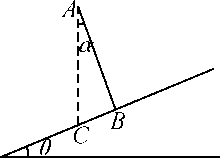
\includegraphics[width=1in,height=0.71875in]{media/image109.png}\end{center}

A.$\alpha$=$\theta$ B.$\alpha=\dfrac{\theta}{2}$

C.$\alpha$=2$\theta$ D.$\alpha=\dfrac{\theta}{3}$

\begin{center}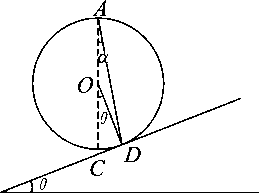
\includegraphics[width=1.17708in,height=0.875in]{media/image110.png}\end{center}
\newpage
\section{牛顿运动定律的综合应用}


1.超重和失重

(1)实重与视重

\ding{172}实重:物体实际所受的重力,与物体的运动状态\_\_无关\_\_.

\ding{173}视重:当物体挂在弹簧测力计下或放在水平台秤上时,弹簧测力计或台秤的\_\_示数\_\_称为视重;视重大小等于弹簧测力计所受物体的\_\_拉力\_\_或台秤所受物体的\_\_压力\_\_.

(2)超重、失重和完全失重的比较

\begin{longtable}[]{@{}m{1.6cm}m{4.7cm}m{4.7cm}m{3.5cm}@{}}
\toprule
& 超重现象 & 失重现象 & 完全失重现象\tabularnewline
\midrule
\endhead
概念 &
物体对支持物的压力(或对悬挂物的拉力)大于物体所受重力的现象 &
物体对支持物的压力(或对悬挂物的拉力)小于物体所受重力的现象 &
物体对支持物的压力(或对悬挂物的拉力)等于零的现象\tabularnewline
产生条件& 物体的加速度方向竖直向上 &物体的加速度方向竖直向下&物体的加速度方向竖直向下,大小a=g \tabularnewline
原理方程& \begin{minipage}[t]{0.22\columnwidth}\raggedright
F-mg=ma

F=m(g+a)\strut
\end{minipage} & \begin{minipage}[t]{0.22\columnwidth}\raggedright
mg-F=ma

F=m(g-a)\strut
\end{minipage} & \begin{minipage}[t]{0.22\columnwidth}\raggedright
mg-F=ma

F=0\strut
\end{minipage}\tabularnewline
运动状态 & 加速上升或减速下降 &
加速下降或减速上升 &
以a=g加速下降或减速上升\tabularnewline
\bottomrule
\end{longtable}

2.连接体问题

(1)整体法和隔离法

\ding{172}整体法

当连接体内(即系统内)各物体的\_\_加速度\_\_相同时,可以把系统内的所有物体看成一个\_\_整体\_\_,分析其受力和运动情况,运用牛顿第二定律对\_\_整体\_\_列方程求解的方法.

\ding{173}隔离法

当求系统内物体间相互作用的\_\_内力\_\_时,常把某个物体从系统中\_\_隔离\_\_出来,分析其受力和运动情况,再用牛顿第二定律对\_\_隔离\_\_出来的物体列方程求解的方法.

(2)动力学图象

\ding{172}三种图象:v-t图象、a-t图象、F-t图象.

\ding{173}图象间的联系:加速度是联系v-t图象与F-t图象的桥梁.

\newpage
\subsection{对超重和失重的理解}

{[}例1{]}广州塔,昵称小蛮腰,总高度达600米,游客乘坐观光电梯大约一分钟就可以到达观光平台.若电梯简化成只受重力与绳索拉力,已知电梯在t=0时由静止开始上升,a-t图象如图所示,则下列相关说法正确的是( D )

\begin{center}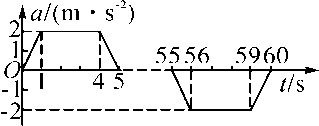
\includegraphics[width=1.44792in,height=0.57292in]{media/image116.png}\end{center}

A.t=4.5 s时,电梯处于失重状态

B.5~55 s时间内,绳索拉力最小

C.t=59.5 s时,电梯处于超重状态

D.t=60 s时,电梯速度恰好为零
\begin{solution}
	利用a-t图象可判断t=4.5
s时,电梯有向上的加速度,电梯处于超重状态,则选项A错误;0~5
s时间内,电梯处于超重状态,拉力\textgreater 重力,5~55
s时间内,电梯处于匀速上升过程,拉力=重力,55~60
s时间内,电梯处于失重状态,拉力\textless 重力,综上所述,选项B、C错误;因a-t图线与t轴所围的``面积''代表速度改变量,而图中横轴上方的``面积''与横轴下方的``面积''相等,则电梯的速度在t=60
s时为零,选项D正确.
\end{solution}

\begin{center}
\includegraphics[width=0.70833in,height=0.125in]{media/image37.png}

\textbf{判断超重和失重现象的三个角度}
\end{center}


(1)从受力的角度判断

当物体受向上的拉力(或支持力)大于重力时,物体处于超重状态;小于重力时处于失重状态,等于零时处于完全失重状态.

(2)从加速度的角度判断

当物体具有向上的加速度时处于超重状态,具有向下的加速度时处于失重状态,向下的加速度为重力加速度时处于完全失重状态.

(3)从速度变化角度判断

\ding{172}物体向上加速或向下减速时,超重;

\ding{173}物体向下加速或向上减速时,失重.
\newpage
\subsection{动力学中的图象问题}

\begin{longtable}[]{@{}m{2cm}m{13cm}@{}}
\toprule
图象类型 & 图象的意义\tabularnewline
\midrule
\endhead
v-t图象 &
根据图象的斜率判断加速度的大小和方向进而根据牛顿第二定律求解合外力\tabularnewline
F-a图象 &
首先要根据具体的物理情景,对物体进行受力分析,然后根据牛顿第二定律推导出两个量间的函数关系式,根据函数关系式结合图象,明确图象的斜率、截距或面积的意义,从而由图象给出的信息求出未知量\tabularnewline
a-t图象 &
要注意加速度的正负,正确分析每一段的运动情况,然后结合物体受力情况根据牛顿第二定律列方程\tabularnewline
F-t图象 &
要结合物体受到的力,根据牛顿第二定律求出加速度,分析每一时间段的运动性质\tabularnewline
\bottomrule
\end{longtable}

{[}例2{]}(多选)2012年11月,``歼15''舰载机在``辽宁号''航空母舰上着舰成功,图甲为利用阻拦系统让舰载机在飞行甲板上快速停止的原理示意图.飞机着舰并成功钩住阻拦索后,飞机的动力系统立即关闭,阻拦系统通过阻拦索对飞机施加一作用力,使飞机在甲板上短距离滑行后停止.某次降落,以飞机着舰为计时零点,飞机在t=0.4
s时恰好钩住阻拦索中间位置,其着舰到停止的速度---时间图线如图乙所示.假如无阻拦索,飞机从着舰到停止需要的滑行距离约为1
000 m.已知航母始终静止,重力加速度的大小为g,则( AC )

\begin{center}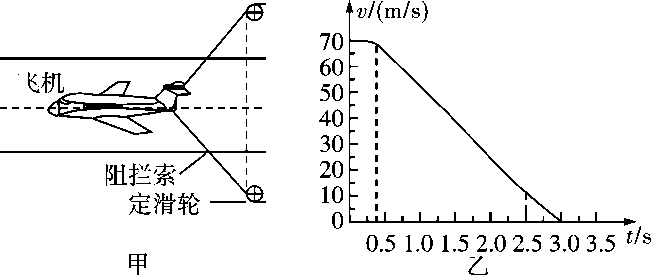
\includegraphics[width=2.95833in,height=1.25in]{media/image117.png}\end{center}

A.从着舰到停止,飞机在甲板上滑行的距离约为无阻拦索时的$\dfrac{1}{10}$

B.在0.4~2.5 s时间内,阻拦索的张力几乎不随时间变化

C.在滑行过程中,飞行员所承受的加速度大小会超过2.5g

D.在0.4~2.5 s时间内,阻拦系统对飞机做功的功率几乎不变

{[}思维导引{]}能正确识图,并从图象中提取所需的信息,是解答此类问题的关键,本题的分析思路具有一定的代表性,逻辑流程如下:

\begin{center}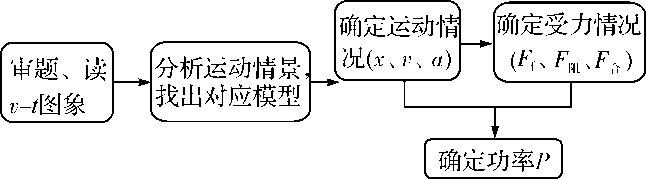
\includegraphics[width=2.9375in,height=0.8125in]{media/image118.png}\end{center}
\newpage
\subsection{连接体问题}

\begin{center}
\includegraphics[width=0.70833in,height=0.125in]{media/image13.png}

\textbf{涉及整体法和隔离法的具体类型}
\end{center}


(1)通过滑轮和绳的连接体问题:若要求绳的拉力,一般都必须采用隔离法.绳跨过定滑轮,连接的两物体虽然加速度大小相同但方向不同,故采用隔离法.

(2)水平面上的连接体问题:这类问题一般多是连接体(系统)中各物体保持相对静止,即具有相同的加速度.解题时,一般整体法、隔离法交替应用.

(3)斜面体与上面物体组成的系统的问题:当物体具有沿斜面方向的加速度,而斜面体相对于地面静止时,解题时一般采用隔离法分析.

{[}例3{]}(多选)如图所示,质量为$m_2$的物体,放在沿平直轨道向左行驶的车厢底板上,并用竖直细绳通过光滑的定滑轮连接质量为$m_1$的物体.当车向左匀加速运动时,与物体$m_1$相连接的绳与竖直方向成$\theta$角,$m_2$与车厢相对静止.则( BD )

\begin{center}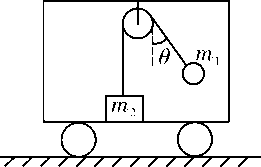
\includegraphics[width=1.1875in,height=0.76042in]{media/image119.png}\end{center}

A.车厢的加速度为 $g\sin\theta$

B.绳对物体$m_1$的拉力T为$\dfrac{m_1g}{\cos\theta}$

C.地板对物体$m_2$的支持力$F_N=(m_2-m_1)g$

D.物体$m_2$所受底板的摩擦力 $F_f=m_2g\tan\theta$
\begin{solution}
	以物体$m_1$为研究对象,分析受力情况如图甲所示,根据牛顿第二定律得$m_1g\tan\theta=m_1a$,得$a=g\tan \theta$,则车厢的加速度也为$g\tan\theta$.绳对物体$m_1$的拉力$T=\dfrac{m_1g}{\cos\theta}$,故选项A错误,B正确;以物体$m_2$为研究对象,分析其受力情况如图乙所示,根据牛顿第二定律有$F_N=m_2g-T=m_2g-\dfrac{m_1g}{\cos\theta}$,$F_f=m_2a=m_2g\tan\theta$.故选项C错误,D正确.
\end{solution}


\begin{center}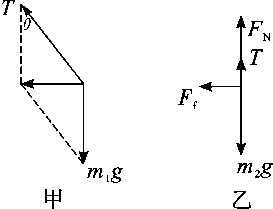
\includegraphics[width=1.23958in,height=0.94792in]{media/image120.png}\end{center}
\begin{center}
\includegraphics[width=0.70833in,height=0.125in]{media/image25.png}\end{center}
分析连接体问题的思路

\begin{center}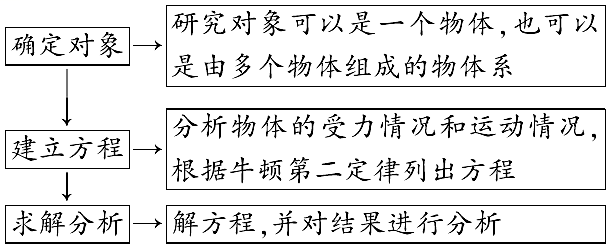
\includegraphics[width=2.65625in,height=1.08333in]{media/image121.png}\end{center}
\subsection{传送带模型}

传送带模型问题包括水平传送带问题和倾斜传送带问题.

1.水平传送带问题

求解的关键在于对物体所受的摩擦力进行正确的分析判断.物体的速度与传送带速度相等的时刻就是物体所受摩擦力发生突变的时刻.

2.倾斜传送带问题

求解的关键在于分析清楚物体与传送带的相对运动情况,从而确定其是否受到滑动摩擦力作用.当物体速度与传送带速度相等时,物体所受的摩擦力有可能发生突变.

{[}例4{]}(2018·山东济南重点中学联考)如图甲所示,水平传送带沿顺时针方向匀速运转.从传送带左端P先后由静止轻轻放上三个物体A、B、C,物体A经$t_A=9.5s$到达传送带另一端Q,物体B经$t_B=10s$到达传送带另一端Q,若释放物体时刻作为t=0时刻,分别作出三物体的v-t图象如图乙、丙、丁所示.求:

\begin{center}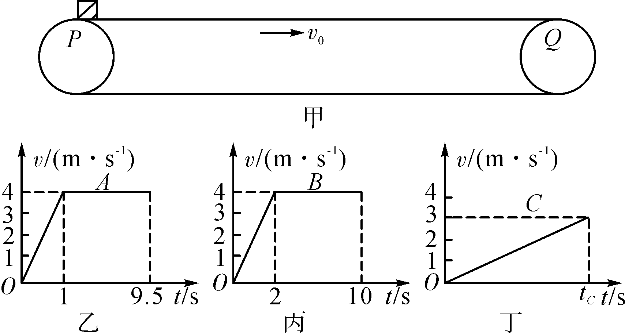
\includegraphics[width=2.84375in,height=1.51042in]{media/image122.png}\end{center}

(1)传送带的速度大小$v_0$;

(2)PQ的长度L;

(3)物体A、B、C与传送带间的动摩擦因数;

(4)物体C从传送带左端P到右端Q所用的时间$t_C$.
\begin{solution}
	(1)4 m/s (2)36 m (3)0.4 0.2 0.012 5 (4)24 s
\end{solution}

\begin{center}
\includegraphics[width=0.70833in,height=0.125in]{media/image13.png}

\textbf{滑块在水平传送带上运动常见的三个情景}
\end{center}


\begin{longtable}[]{@{}m{1cm}m{2.5cm}m{10cm}@{}}
\toprule
项目 & 图示 & 滑块可能的运动情景\tabularnewline
\midrule
\endhead

情
景
1
&
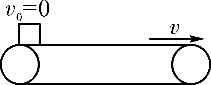
\includegraphics[width=0.95833in,height=0.38542in]{media/image123.png}& 
(1)可能一直加速

(2)可能先加速后匀速\tabularnewline
情
景
2
&
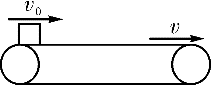
\includegraphics[width=0.95833in,height=0.38542in]{media/image124.png}
 &
(1)$\mathrm v_0$\textgreater v时,可能一直减速,也可能先减速再匀速\tabularnewline

情
景
3
& 
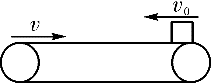
\includegraphics[width=0.95833in,height=0.375in]{media/image125.png}
& 
(1)传送带较短时,滑块一直减速达到左端

(2)传送带较长时,滑块还要被传送带传回右端.

其中$\mathrm v_0$\textgreater v返回时速度为v,当$\mathrm v_0$\textless v返回时速度为$\mathrm v_0$\strut
\tabularnewline
\bottomrule
\end{longtable}
\newpage
{[}例5{]}如图所示,倾角为$\theta=30^\circ$的皮带运输机的皮带始终绷紧,且以恒定速度v=2.5
m/s运动,两轮相距$L_{AB}=5 m$,将质量m=1
kg的物体无初速度地轻轻放在A处,若物体与皮带间的动摩擦因数$\mu$=(取g=10
$g=10m/s^2$),物体从A运动到B共需多长时间?

\begin{center}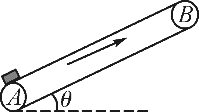
\includegraphics[width=0.90625in,height=0.51042in]{media/image126.png}\end{center}
\begin{solution}
2.5 s

	第一阶段,物块向上匀加速运动,由牛顿第二定律有

$\mu mg\cos \theta-mg\sin \theta=ma_1$,

代入数据求得$a_1=2.5 m/s^2$.

根据匀变速直线运动规律得$v=a_1t_1$,$x_1=t_1$,

代入数据求得$t_1=1 s$,$x_1=1.25 m$.

第二阶段,由于$\mu>\tan \theta$,故物体向上匀速运动.

$L_{AB}-x_1=vt_2$,

$t_2=1.5 s$.

总时间$t=t_1+t_2=2.5 s$.


\end{solution}


\begin{center}
\includegraphics[width=0.70833in,height=0.125in]{media/image13.png}

\textbf{滑块在倾斜传送带上运动常见的四个情景}
\end{center}


\begin{longtable}[]{@{}m{1cm}m{2.5cm}m{5cm}@{}}
\toprule
项目 & 图示 & 滑块可能的运动情景\tabularnewline
\midrule
\endhead

情
景
1
&
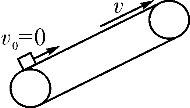
\includegraphics[width=0.86458in,height=0.48958in]{media/image127.png}
&
(1)可能一直加速

(2)可能先加速后匀速
\tabularnewline

情
景
2
&
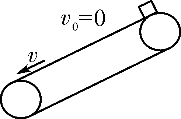
\includegraphics[width=0.82292in,height=0.54167in]{media/image128.png}
&
(1)可能一直加速

(2)可能先加速后减速

(3)可能先以$a_1$加速后以$a_2$加速
\tabularnewline

情
景
3
&
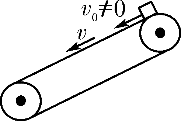
\includegraphics[width=0.82292in,height=0.55208in]{media/image129.png}
&
(1)可能一直加速

(2)可能先加速后匀速

(3)可能一直减速

(4)可能先以$a_1$加速后以$a_2$加速
\tabularnewline

情
景
4
&
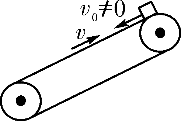
\includegraphics[width=0.82292in,height=0.55208in]{media/image130.png}
&
(1)可能一直加速

(2)可能一直减速

(3)可能先减速后反向加速

(4)可能一直减速
\tabularnewline
\bottomrule
\end{longtable}
\newpage
\subsection{滑块------木板模型}

1.模型特点:滑块(视为质点)置于木板上,滑块和木板均相对地面运动,且滑块和木板在摩擦力的相互作用下发生相对滑动.

2.位移关系:滑块由木板一端运动到另一端的过程中,滑块和木板同向运动时,位移之差$\Delta x=x_1-x_2=L$(板长);滑块和木板反向运动时,位移之和$\Delta x=x_2+x_1=L$.

\begin{center}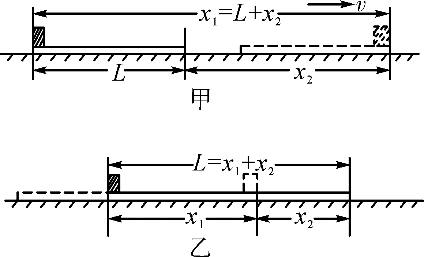
\includegraphics[width=1.92708in,height=1.16667in]{media/image131.png}\end{center}

{[}例6{]}一长木板在水平地面上运动,在t=0时刻将一相对于地面静止的物块轻放到木板上,以后木板运动的速度---时间图象如图所示.已知物块与木板的质量相等,物块与木板间及木板与地面间均有摩擦.物块与木板间的最大静摩擦力等于滑动摩擦力,且物块始终在木板上,取重力加速度的大小$g=10m/s^2$.求:

(1)物块与木板间、木板与地面间的动摩擦因数;

(2)从t=0时刻到物块与木板均停止运动时,物块相对于木板的位移的大小.

\begin{center}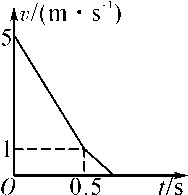
\includegraphics[width=0.85417in,height=0.88542in]{media/image132.png}\end{center}
\begin{solution}
	(1)0.20 0.30 (2)1.125 m
\end{solution}
\begin{center}
\includegraphics[width=0.70833in,height=0.125in]{media/image25.png}

\textbf{``滑块------滑板''模型问题的分析思路}
\end{center}


\begin{center}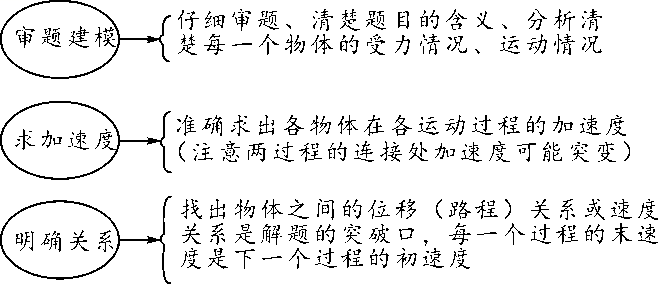
\includegraphics[width=3in,height=1.29167in]{media/image133.png}\end{center}
\newpage
\begin{problemset}
	\item \textbf{反向ma}
	
	\qquad 多个物体受力分析中,整体法的优越性不言而喻,但是应用此方法的条件较为苛刻:加速度相同。当两个物体加速度不同时,我们通常隔离后分析受力情况,此时分析过程冗长且耗时。反向ma则可以解决这一矛盾,下面以例3.1演示该方法的优越性。
	\begin{example}
		(2018·四川高考模拟)质量为m的滑块沿放在水平地面上质量也为m的倾角为θ的固定光滑斜面下滑时,斜面对地面的压力大小为$F_1$;当滑块和固定斜面接触面间有摩擦且滑块沿斜面匀速下滑时,斜面对地面的压力大小为$F_2$。则$F_1:F_2$等于
		
		    A.$(1+\cos^2\theta):2$
    		
    		B.$(1+\sin^2\theta):2$  
    
    		C.$1:1    $     
    
    		D.$(1+\sin^2\theta):2$ 
    		\begin{solution}A
    		
    		斜面不固定时:
    		
			如图建立直角坐标系,给滑块施加沿x轴反方向向上$\theta$的力,大小为$mg\sin\theta$.
\begin{center}
	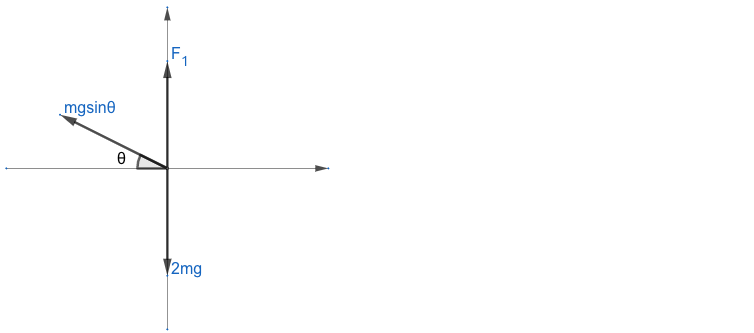
\includegraphics[width=5in]{media/31.png}
\end{center}

				此时有$a_{\text{滑块}}=a_{\text{斜面}}$,整体受力分析得
			\begin{equation}
				F_1=2mg-mg\sin\theta
			\end{equation}
			斜面固定时:
			\begin{equation}
				F_2=2mg
			\end{equation}
			
			联立公式(3.1)(3.2)得
			\begin{equation}
				F_1:F_2=(1+\cos^2\theta):2
			\end{equation}
			
    		\end{solution}
	\end{example}
	\newpage
	\item \textbf{质量分配}
	\begin{itemize}
		\item 简单模型
		\begin{conclusion}
			外力F作用在物体M上,M可任意分成2部分$m_A$,$m_B$。$m_A$与$m_B$无相对位移。若二者之间的力T与外力F共线且F作用在$m_B$上,则$T=\dfrac{m_A}{M}F=\dfrac{m_A}{m_A+m_B}F$
		\begin{proof}
		
			整体受力分析
			\begin{equation}
				F=(m_A+m_B)a
			\end{equation}
			隔离$m_A$受力分析
			\begin{equation}
				T=m_Aa
			\end{equation}
			联立公式(3.4)(3.5)得
			\begin{equation}
				T=\dfrac{m_A}{m_A+m_B}F
			\end{equation}
		\end{proof}
		\end{conclusion}
		\item 质量分配+伽利略变换(\ding{72}\ding{72}\ding{72})
		
		高中适用该方法的题目的受力情况一般相对复杂,这种情况下可以将上述条件拓展:
		\begin{conclusion}
			$m_A$,$m_B$分别受到外力$F_A$,$F_B$的作用且满足条件(3.7)
			\begin{equation}
			\dfrac{F_A}{m_A}=\dfrac{F_B}{m_B}
			\end{equation}
			$T$满足公式(3.6)
		\end{conclusion}

		
		\begin{proof}
			整体受力分析
			\begin{equation}
				F+F_A+F_B=(m_A+m_B)a
			\end{equation}
			隔离$m_A$受力分析
			\begin{equation}
				T+F_A=m_Aa
			\end{equation}
			联立公式(3.8)(3.9)得
			\begin{equation}
				T=\dfrac{m_A}{m_A+m_B}F
			\end{equation}
		\end{proof}
		更具艺术性的证明是直接应用公式(3.7)中的加速度,通过伽利略变换即可将该模型转化为简单模型
	\end{itemize}
	\newpage
	\item 板块模型
	
	本小节将会应用质量分配公式对板块模型进行简单的分析
\begin{center}
	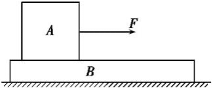
\includegraphics[width=2in]{media/33.png}
\end{center}
	如图所示,已知:$m_A$,$m_B$,F,AB间摩擦系数为$\mu _1$,B与地面摩擦系数为$\mu _2$

	定义:$a_c$为共同加速度
	\begin{itemize}
		\item $\mu 2=0$
		\begin{itemize}
			\item $0<F<F_{\max }$
			
				$F=\left(m_{A}+m_{B}\right) a_{c} $

				$f=\dfrac{m_{B}}{m_{A}+m_{B}} F=\mu_{1} m_{A} g \Rightarrow F_{\max }=\dfrac{\mu_{1} m_{A} g\left(m_{A}+m_{B}\right)}{m_{B}}$
			\item $F_{\max }<F<\infty$
			
				$\left\{\begin{array}{c}F-\mu_{1} m_{A} g=m_{A} a_{A} \\ \mu_{1} m_{A} g=m_{B} a_{B}\end{array}\right.$
		\end{itemize}
		\item $\mu 2\neq 0$且$\mu_{1} m_{A} g<\mu_{2}\left(m_{A}+m_{B}\right) g$
		\begin{itemize}
			\item $0<F<\mu_{1} m_{A} g$
			
				$v_{A}=v_{B}=0$
			\item $\mu_{1} m_{A} g<F<\infty$
			
				$\left\{\begin{array}{c}F-\mu_{1} m_{A} g=m_{A} a_{A} \\ a_{B}=0\end{array}\right.$
		\end{itemize}
		\item $\mu 2\neq 0$且$\mu_{1} m_{A} g>\mu_{2}\left(m_{A}+m_{B}\right) g$
		\begin{itemize}
			\item $0<F<\mu_{2}\left(m_{A}+m_{B}\right) g$
				
				$v_{A}=v_{B}=0$
			\item $\mu_{2}\left(m_{A}+m_{B}\right) g<F<F_{\max }$
				
				$F-\mu_{2}\left(m_{A}+m_{B}\right) g=\left(m_{A}+m_{B}\right) a_{c}$
				
				$f=\dfrac{m_{B} F+m_{A}\left[\mu_{2}\left(m_{A}+m_{B}\right) g\right]}{m_{A}+m_{B}}=\mu_{1} m_{A} g \Rightarrow F_{\max }=\dfrac{\left(\mu_{1}-\mu_{2}\right) m_{A} g\left(m_{A}+m_{B}\right)}{m_{B}}$
			\item $F_{\max }<F<\infty$
				
				$\left\{\begin{array}{c}F-\mu_{1} m_{A} g=m_{A} a_{A} \\ \mu_{1} m_{A} g-\mu_{2}\left(m_{A}+m_{B}\right) g=m_{B} a_{B}\end{array}\right.$
		\end{itemize} 
			
	\end{itemize}
	\begin{example}
		若满足最后一种情况,且$F$随时间$t$均匀增大:$F=kt$
\begin{center}
	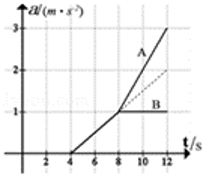
\includegraphics[width=2in]{media/34.png}
\end{center}
	$F-\mu_{2}\left(m_{A}+m_{B}\right) g=\left(m_{A}+m_{B}\right) a_{c} \Rightarrow a_{c}=\dfrac{F}{\left(m_{A}+m_{B}\right)}-\mu_{2} g$
	
	$F-\mu_{1} m_{A} g=m_{A} a_{A} \Rightarrow a_{A}=\dfrac{F}{m_{A}}-\mu_{1} g$
	
	$\mu_{1} m_{A} g-\mu_{2}\left(m_{A}+m_{B}\right) g=m_{B} a_{B} \Rightarrow a_{B}=\dfrac{\left(\mu_{1}-\mu_{2}\right) m_{A} g}{m_{B}}-\mu_{2} g$
	\end{example}
	\newpage
	\item 传送带模型
	
	太多了,懒得迁移
\end{problemset}

